\documentclass[11pt,a4paper]{article}

\usepackage[a4paper,top=0.85in,bottom=0.85in,left=0.95in,right=0.95in]{geometry}
\usepackage{graphicx}
\usepackage{amsmath}
\usepackage{booktabs}
\usepackage{array}
\usepackage{xcolor}
\usepackage{tabularx}
\usepackage{enumitem}
\usepackage{caption}
\usepackage{titlesec}
\usepackage{listings}
\usepackage{float}
\usepackage[hidelinks]{hyperref}
\usepackage{fancyhdr}
\usepackage{microtype}

% Nature-light palette
\definecolor{cTitle}{HTML}{2C3E50}
\definecolor{cAccent}{HTML}{C5732D}
\definecolor{cSlate}{HTML}{6B7280}
\definecolor{cCodeBg}{HTML}{F6F4EF}
\definecolor{cKeyword}{HTML}{2563EB}
\definecolor{cString}{HTML}{B85A47}
\definecolor{cComment}{HTML}{3E8E5E}
\definecolor{cRule}{HTML}{D5D0C4}

\titleformat{\section}{\large\bfseries\color{cTitle}}{\thesection.}{0.5em}{}
\titleformat{\subsection}{\normalsize\bfseries\color{cTitle!85!black}}{\thesubsection}{0.5em}{}
\titlespacing{\section}{0pt}{8pt}{4pt}
\titlespacing{\subsection}{0pt}{6pt}{3pt}

\captionsetup{font=small,labelfont={bf,color=cTitle},skip=4pt}
\graphicspath{{../figures/}}

\pagestyle{fancy}
\fancyhf{}
\fancyhead[L]{\small\color{cSlate} EBU5503 -- Hotel Booking \& Management System -- Group 13}
\fancyhead[R]{\small\color{cSlate} \thepage}
\renewcommand{\headrulewidth}{0.4pt}

\lstdefinestyle{sqlstyle}{
    backgroundcolor=\color{cCodeBg},
    basicstyle=\ttfamily\scriptsize\color{black!85},
    keywordstyle=\color{cKeyword}\bfseries,
    commentstyle=\color{cComment}\itshape,
    stringstyle=\color{cString},
    showstringspaces=false,
    breaklines=true,
    frame=single,
    rulecolor=\color{cSlate!50},
    framerule=0.3pt,
    captionpos=b,
    xleftmargin=6pt,
    aboveskip=4pt,
    belowskip=4pt,
    morekeywords={SELECT,FROM,WHERE,JOIN,LEFT,RIGHT,INNER,ON,AND,OR,NOT,IN,EXISTS,GROUP,BY,HAVING,ORDER,DESC,ASC,AS,CASE,WHEN,THEN,ELSE,END,WITH,UNION,COUNT,SUM,AVG,MAX,MIN,COALESCE,DATEDIFF,DATE_FORMAT,ROUND,RANK,ROW_NUMBER,PARTITION,OVER,CREATE,VIEW,TABLE,PRIMARY,KEY,FOREIGN,REFERENCES,DEFAULT,NULL,CHECK,UNIQUE,INDEX,ENUM,VARCHAR,INT,DATETIME,DATE,DECIMAL,BOOLEAN,TEXT,USE,LIMIT,DISTINCT,LEAST,GREATEST,USING,IS}
}

\setlength{\parskip}{2pt}
\setlength{\parindent}{1.2em}

\begin{document}

% ============================ Title ============================
\begin{center}
\vspace{-10pt}
{\color{cTitle}\LARGE\bfseries Hotel Booking \& Management System\par}
\vspace{4pt}
{\normalsize\itshape A Normalised Relational Design with a Database-Driven Pricing Agent\par}
\vspace{8pt}
{\small EBU5503 Database Systems --- Group Coursework Report (2025/26)\par}
{\small\color{cSlate} Scenario 2: Hotel Reservation \& Management \quad|\quad \textbf{Group 13} \quad|\quad 20 May 2026\par}

\vspace{10pt}
{\footnotesize\color{black!75}
\begin{tabular}{@{}l@{\hspace{2em}}l@{\hspace{2em}}l@{}}
Xinke Lyu \quad 241119389 &
Hao Wang \quad 241119563 &
Yiju Huang \quad 241119116 \\[1pt]
Haoxiang Fan \quad 241119035 &
Zelin Li \quad 241119161 &
Xinyu Li \quad 241119183 \\[1pt]
\multicolumn{3}{c}{Xinzhu Liu \quad 241119312} \\
\end{tabular}\par}
\end{center}
\vspace{-2pt}{\color{cRule}\hrule height 0.6pt}\vspace{6pt}

% ============================ 1. Requirements ============================
\section{Detailed Requirements and Assumptions}

\subsection{Scope and basic requirements}
The system records the four data domains mandated by Scenario~2 --
\textbf{guests}, \textbf{rooms}, \textbf{bookings/reservations} and
\textbf{payments} -- together with the operational artefacts a non-trivial
Property Management System inevitably accretes around them. A booking
belongs to exactly one guest, may span multiple rooms over arbitrary date
ranges, and is settled by one or more payment transactions including
deposits, settlements and refunds.

\subsection{Additional requirements (creative extensions)}
Five extensions are introduced, each justified by a concrete operational need
rather than an academic flourish.

\begin{tabularx}{\linewidth}{@{}p{3.2cm} X@{}}
\toprule
\textbf{Extension} & \textbf{Justification and real-world mapping} \\
\midrule
Loyalty Program       & Tiered membership (Bronze/Silver/Gold/Platinum) mirrors Marriott Bonvoy and Hilton Honors; supports retention analytics (Q4, Q11). \\
Dynamic Pricing Rule  & Event- and season-based multipliers (Christmas, Spring Festival, Summer, weekdays) move the design from static rate cards to revenue-managed pricing. \\
Room Type abstraction & Separates physical room from pricing category, removing the update anomaly that would arise from storing rate per row of \textsc{Room} (2NF). \\
Department \& Staff   & Models internal organisation, prerequisite for any task-assignment analytics. \\
Task Log              & Records cleaning, maintenance and inspection per (Staff, Room, Task\_Type); a true ternary relationship that underpins Q6/Q8. \\
\bottomrule
\end{tabularx}

\subsection{Key assumptions}
\begin{itemize}[leftmargin=*,topsep=2pt,itemsep=1pt]
    \item A booking can span multiple rooms with independent check-in/out windows.
    \item Payments may be partial deposits, full settlements or cancellation refunds; status is one of \texttt{Completed/Pending/Refunded/Failed}.
    \item Loyalty enrolment is optional and at most one record per guest (1:1).
    \item Pricing rules are date-windowed and globally applicable; \texttt{Priority} resolves overlapping windows deterministically.
    \item Same-room overlap prevention is enforced by application logic plus Q12 (self-join audit); SQL alone cannot natively express range non-overlap.
\end{itemize}

% ============================ 2. EER ============================
\section{Conceptual Schema (EER Design)}

The conceptual model comprises \textbf{11 entities} arranged into four functional
domains: \emph{customer} (Guest, Loyalty\_Program), \emph{inventory} (Room\_Type,
Room, Dynamic\_Pricing\_Rule), \emph{transactional} (Booking, Booking\_Room\_Detail,
Payment) and \emph{operational} (Department, Staff, Task\_Log). The
Workbench-exported EER diagram in Figure~\ref{fig:eer} renders the layout, and the
prose below names every relationship type explicitly so that the design is
auditable without recourse to the visual.

\begin{figure}[H]
\centering
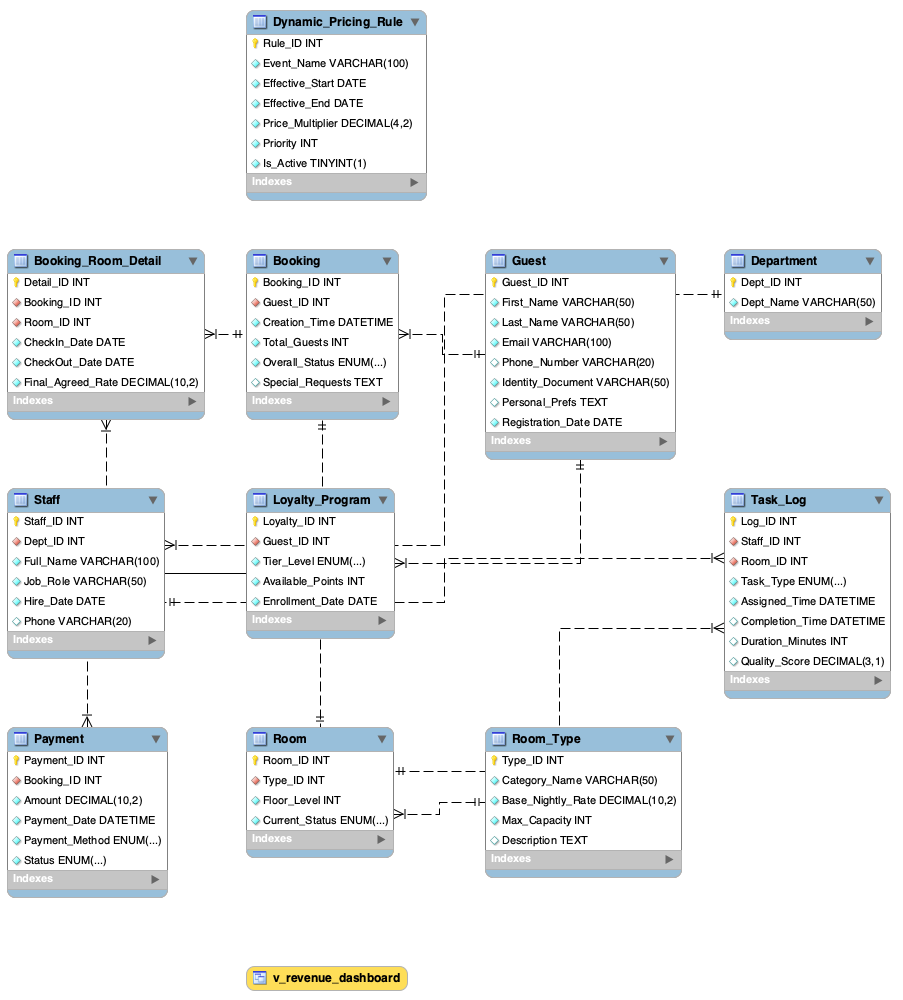
\includegraphics[width=0.95\linewidth]{fig1_eer_overview.png}
\caption{EER diagram of the Hotel Booking \& Management System, exported from MySQL Workbench Reverse Engineer. Crow's-foot cardinalities are visible at each endpoint; \textsc{Booking\_Room\_Detail} is the associative entity that resolves the M:N relationship between \textsc{Booking} and \textsc{Room}, and \textsc{Task\_Log} resolves the ternary relationship over (Staff, Room, Task\_Type).}
\label{fig:eer}
\end{figure}

\textbf{Relationship inventory.}
(i)~\textsc{Booking}--\textsc{Room} is M:N, decomposed by the associative entity
\textsc{Booking\_Room\_Detail} that carries per-room check-in/out dates and the
\emph{agreed} nightly rate (which may differ from base after pricing rules).
(ii)~(\textsc{Staff}, \textsc{Room}, \textsc{Task\_Type}) form a true ternary
relationship realised as \textsc{Task\_Log}.
(iii)~\textsc{Guest}--\textsc{Loyalty\_Program} is optional 1:1 on the guest side
(\texttt{UNIQUE} on \texttt{Guest\_ID}).
(iv)~\textsc{Guest}--\textsc{Booking} is 1:N; \textsc{Booking}--\textsc{Payment} is 1:N.
(v)~\textsc{Department}--\textsc{Staff} is 1:N.
(vi)~\textsc{Room\_Type}--\textsc{Room} is 1:N.
(vii)~\textsc{Dynamic\_Pricing\_Rule} is a deliberately \emph{unrelated} global
entity, consulted by the Pricing Agent at booking time. Decoupling it via the
application layer (rather than a hard FK to \textsc{Booking\_Room\_Detail}) allows
rules to evolve independently of historical bookings -- a design choice that pays
back when discount windows are retired.

% ============================ 3. Schema & Normalisation ============================
\section{Relational Schema and Normalisation}

\subsection{Relational schema}
The conceptual model translates into 11 relations. Underlined attributes are
primary keys, \emph{italicised} attributes are foreign keys, and
\textsuperscript{U} denotes \textsc{Unique}.

\vspace{2pt}
\begin{tabularx}{\linewidth}{@{}lX@{}}
\toprule
\textbf{Relation} & \textbf{Attributes} \\
\midrule
Guest                 & \underline{Guest\_ID}, First\_Name, Last\_Name, Email\textsuperscript{U}, Phone, Identity\_Doc\textsuperscript{U}, Personal\_Prefs, Registration\_Date \\
Loyalty\_Program      & \underline{Loyalty\_ID}, \emph{Guest\_ID}\textsuperscript{U}, Tier\_Level, Available\_Points, Enrollment\_Date \\
Room\_Type            & \underline{Type\_ID}, Category\_Name\textsuperscript{U}, Base\_Nightly\_Rate, Max\_Capacity, Description \\
Room                  & \underline{Room\_ID}, \emph{Type\_ID}, Floor\_Level, Current\_Status \\
Booking               & \underline{Booking\_ID}, \emph{Guest\_ID}, Creation\_Time, Total\_Guests, Overall\_Status, Special\_Requests \\
Booking\_Room\_Detail & \underline{Detail\_ID}, \emph{Booking\_ID}, \emph{Room\_ID}, CheckIn\_Date, CheckOut\_Date, Final\_Agreed\_Rate \\
Payment               & \underline{Payment\_ID}, \emph{Booking\_ID}, Amount, Payment\_Date, Payment\_Method, Status \\
Dynamic\_Pricing\_Rule& \underline{Rule\_ID}, Event\_Name, Effective\_Start, Effective\_End, Price\_Multiplier, Priority, Is\_Active \\
Department            & \underline{Dept\_ID}, Dept\_Name\textsuperscript{U} \\
Staff                 & \underline{Staff\_ID}, \emph{Dept\_ID}, Full\_Name, Job\_Role, Hire\_Date, Phone \\
Task\_Log             & \underline{Log\_ID}, \emph{Staff\_ID}, \emph{Room\_ID}, Task\_Type, Assigned\_Time, Completion\_Time, Duration\_Minutes, Quality\_Score \\
\bottomrule
\end{tabularx}

\subsection{Normalisation walkthrough}
\textbf{1NF.} All attributes are atomic; the early-draft monolithic
\texttt{LOG(guest,~room,~payment)} relation conflated three concerns and was
split into \textsc{Booking}, \textsc{Booking\_Room\_Detail} and \textsc{Payment}.
\textbf{2NF.} No non-key attribute depends on part of a composite key. The
candidate violation -- \texttt{ROOM(Room\_ID, Price, Type, Capacity)} -- was
resolved by abstracting \textsc{Room\_Type}, so that capacity and base rate
depend on \texttt{Type\_ID} rather than on every individual room row.
\textbf{3NF.} No transitive dependencies remain. In particular, \textsc{Payment}
stores only \emph{Booking\_ID} and reaches guest details transitively through
\textsc{Booking}, eliminating the \texttt{Guest\_ID} $\rightarrow$
\texttt{Guest\_Email} transitive that an early sketch carried.
\textbf{BCNF.} Every non-trivial functional dependency has a superkey on its
left-hand side; the schema is therefore in BCNF, and no further decomposition
is required.

% ============================ 4. Sample Data ============================
\section{Sample Data and Empirical Findings}

\subsection{Dataset construction and coverage}
The populated instance contains \textbf{125 rows} across the 11 tables
(Department 5, Staff 8, Room\_Type 5, Room 12, Guest 10, Loyalty\_Program 6,
Pricing\_Rule 4, Booking 15, Booking\_Room\_Detail 18, Payment 12, Task\_Log 15).
The data is deliberately seeded to stress every edge case the query set must
handle: repeat guests (Guests 1 and 2 with multiple bookings), multi-room
bookings (B2, B6, B12), cancellations with refunds (B4, B9), room reuse across
non-overlapping dates (Rooms 101 and 303), a partial-payment \texttt{Pending}
booking (B12), and an open work item with \texttt{NULL} completion (Task 4 --
AC repair, Room 301, unresolved since 10~Jan).

Figure~\ref{fig:violin} shows the per-night revenue distribution by room
category, computed on non-cancelled \texttt{Booking\_Room\_Detail} rows.
Premium suites occupy a noticeably wider rate band; this is the direct
fingerprint of dynamic pricing rules biting hardest on high-demand inventory.
The same distribution, viewed through the lens of payment volume, supports
\textbf{Finding F5}: of the total \$7{,}624 settled through the payment table,
12.37\% is at risk (Pending+Refunded), and Credit-Card transactions average
9.3$\times$ the Cash mean -- premium stays effectively \emph{must} clear card
rails, making terminal reliability a revenue-critical concern.

\begin{figure}[H]
\centering
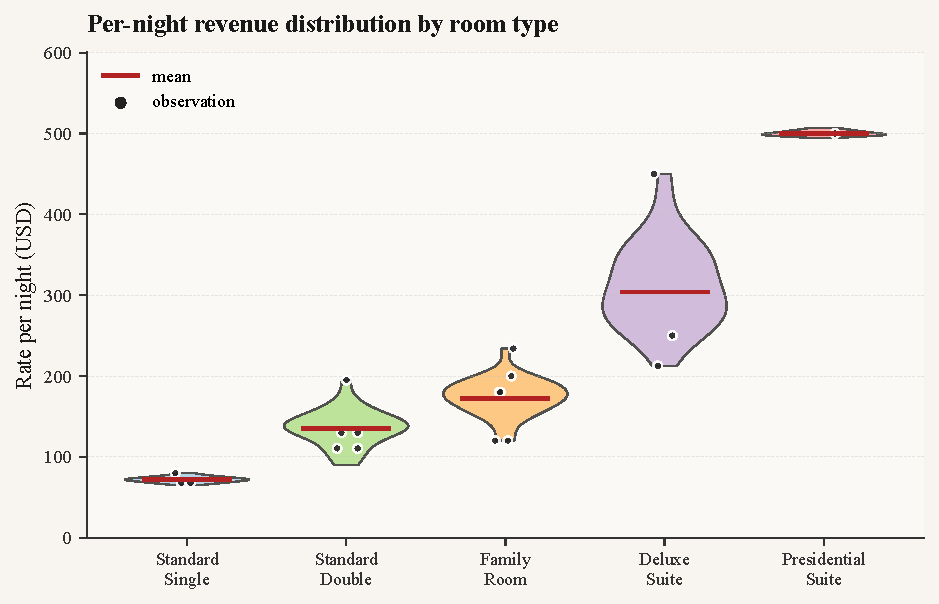
\includegraphics[width=0.85\linewidth]{fig2_violin_revenue.pdf}
\caption{Per-night revenue distribution by room category (non-cancelled details only). Inner quartile lines and overlaid raw points expose how dynamic-pricing rules stretch the rate distribution of premium rooms.}
\label{fig:violin}
\end{figure}

\subsection{Length-of-stay structure}
Figure~\ref{fig:ridge} re-slices the same booking-detail table by occupied
nights per category: Standard Doubles concentrate around 2-3 night stays
while Executive and Presidential Suites exhibit longer-tail behaviour. This
is the structural reason \textbf{Finding F2}'s cancellations (B4 and B9)
hurt disproportionately -- the cancelled inventory is precisely the
long-stay, high-rate tail.

\begin{figure}[H]
\centering
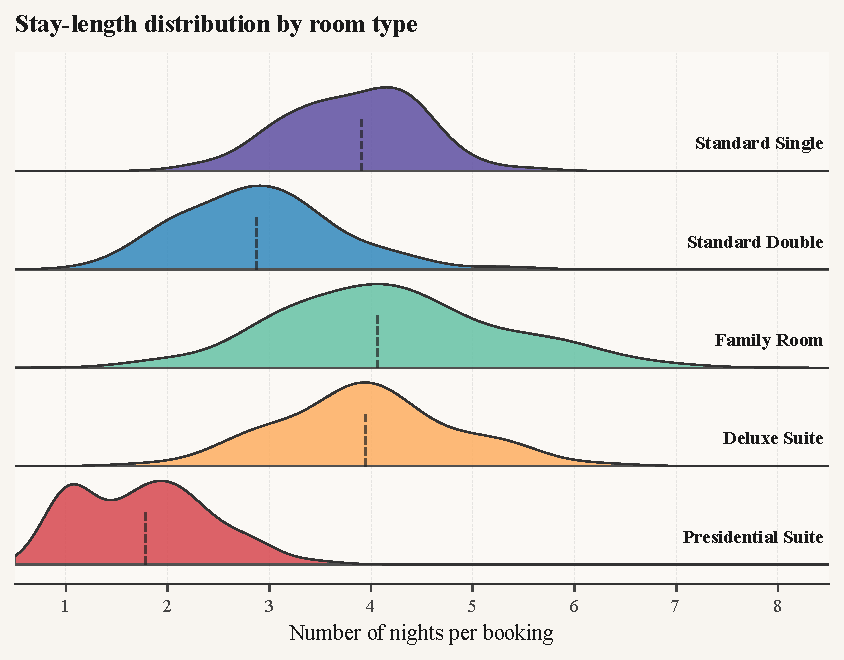
\includegraphics[width=0.70\linewidth]{fig8_ridgeplot_room_status.pdf}
\caption{Ridge plot of stay length (\texttt{CheckOut\_Date}~-~\texttt{CheckIn\_Date}) by room category. Premium categories carry a longer right tail, which is the lever the pricing engine exploits and the risk surface that cancellations expose.}
\label{fig:ridge}
\end{figure}

\subsection{Correlation structure and a loyalty insight}
Figure~\ref{fig:heatmap} reports Pearson correlations across five
\emph{per-booking} metrics on non-cancelled records. At the per-booking grain
the strongest non-trivial pair is \emph{Nightly Rate} $\times$ \emph{Loyalty
Points} at $r \approx 0.41$, indicating that higher-tier members do trade up
to premium rooms. When the data are aggregated to the \emph{per-guest} grain
(total spend across all bookings of a member vs. that member's points
balance), the link weakens to $r = 0.455$ -- still moderate, but
substantially lower than one might expect of a tier system whose primary
purpose is to mirror customer value. Finding~F1 makes this concrete: Silver
members average \$1{,}380 per booking against Bronze's \$400 (a 3.5$\times$
gap). Points reflect historical accumulation; spend reflects current
behaviour. The actionable corollary is that tier upgrades should be triggered
by recent rolling revenue, not lifetime point inertia -- otherwise Bronze
big-spenders (e.g., Guest 10 at \$663 on 800 points) remain under-recognised.

\begin{figure}[H]
\centering
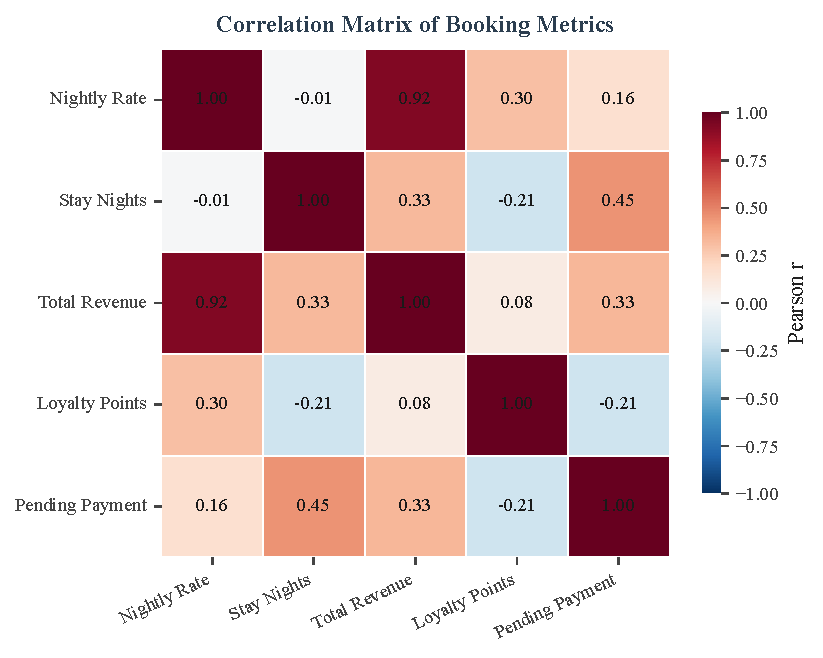
\includegraphics[width=0.55\linewidth]{fig4_heatmap_correlation.pdf}
\caption{Pearson correlation matrix of five booking-level metrics. The moderate \emph{Nightly Rate} $\times$ \emph{Loyalty Points} coupling ($r\approx 0.41$) supports the loyalty subsystem; the weak \emph{Spend} $\times$ \emph{Points} link motivates a rolling-window tier-upgrade rule.}
\label{fig:heatmap}
\end{figure}

% ============================ 5. Queries ============================
\section{SQL Queries and Results}

\subsection{Query catalogue}
The query set comprises \textbf{12 SQL statements} that together reference
\emph{all 11 relations}. They cover multi-table joins, sub-queries
(\texttt{NOT EXISTS}), aggregation with \texttt{HAVING}, window functions
(\texttt{RANK}, \texttt{ROW\_NUMBER}), CTEs, views and a self-join for overlap
detection. The full script lives in \texttt{tests/test\_queries.sql}; the
catalogue below names each query, its business purpose and the relations it
touches.

{\footnotesize
\begin{tabularx}{\linewidth}{@{}llX@{}}
\toprule
\textbf{ID} & \textbf{Purpose} & \textbf{Relations used} \\
\midrule
Q1  & Top spenders                & Guest, Booking, Payment \\
Q2  & Occupancy by room type      & Room\_Type, Room, Booking\_Room\_Detail \\
Q3  & Pricing-rule impact         & Booking\_Room\_Detail, Room\_Type, Pricing\_Rule \\
Q4  & Loyalty-tier ARPU           & Guest, Loyalty\_Program, Booking, Payment \\
Q5  & Date-range availability     & Room, Room\_Type, Booking\_Room\_Detail, Booking \\
Q6  & Department workload         & Department, Staff, Task\_Log \\
Q7  & Revenue by payment method   & Payment, Booking, Booking\_Room\_Detail \\
Q8  & Staff quality (\texttt{HAVING}) & Staff, Task\_Log \\
Q9  & Operational dashboard view  & 7-table \texttt{LEFT JOIN} view \\
Q10 & Monthly cancellation watch  & Booking, Booking\_Room\_Detail \\
Q11 & VIP scoring (CTE + window)  & Guest, Booking, Payment, Loyalty\_Program \\
Q12 & Overlap conflict audit      & Booking\_Room\_Detail (self-join) \\
\bottomrule
\end{tabularx}}

\subsection{Three representative queries}
Q5 illustrates the schema's defensive design. By using \texttt{NOT EXISTS} with a
date-overlap predicate rather than the live \texttt{Room.Current\_Status}, the
system correctly handles \emph{future} reservations on rooms whose current
status is still \texttt{Available}.

\begin{lstlisting}[style=sqlstyle,caption={Q5 -- Date-range availability via \texttt{NOT EXISTS}.}]
SELECT r.Room_ID, rt.Category_Name, r.Floor_Level, rt.Base_Nightly_Rate
FROM Room r JOIN Room_Type rt ON r.Type_ID = rt.Type_ID
WHERE r.Current_Status != 'Maintenance'
  AND NOT EXISTS (
    SELECT 1 FROM Booking_Room_Detail brd
    JOIN Booking b ON brd.Booking_ID = b.Booking_ID
    WHERE brd.Room_ID = r.Room_ID
      AND b.Overall_Status NOT IN ('Cancelled')
      AND brd.CheckIn_Date  < '2026-06-05'
      AND brd.CheckOut_Date > '2026-06-01');
\end{lstlisting}

\textbf{Q1 -- Top spenders} (Guest $\bowtie$ Booking $\bowtie$ Payment) ranks
guests by completed payment volume. The highest single-booking spend is a
family stay over the New Year peak; the cancellation cluster of
\textbf{Finding~F2} is visible immediately upstream as a parallel red ribbon
in Figure~\ref{fig:sankey}, which traces every booking from its guest's
loyalty tier all the way to outcome. Ribbon thickness encodes booking count
and shows the disproportionate share of repeat business held by the top two
tiers.

\begin{figure}[H]
\centering
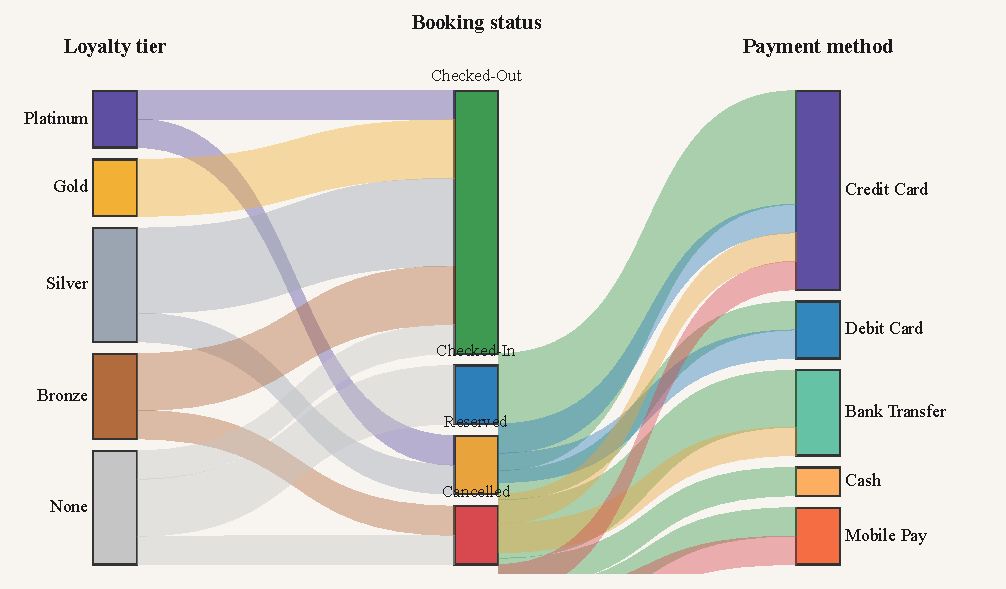
\includegraphics[width=0.95\linewidth]{fig3_sankey_loyalty_flow.pdf}
\caption{Sankey flow: loyalty tier $\rightarrow$ booking status. The red Cancelled branch corresponds to the refunded payments returned by Q10; its narrowness understates the revenue impact (\$2{,}480 lost) because the cancellations concentrate on premium inventory.}
\label{fig:sankey}
\end{figure}

\textbf{Q11 -- VIP scoring} blends total spend, booking frequency and loyalty
tier inside a CTE, producing a defensible 0--100 score:

\begin{lstlisting}[style=sqlstyle,caption={Q11 -- VIP scoring CTE (Guest, Booking, Payment, Loyalty\_Program).}]
WITH customer_metrics AS (
  SELECT g.Guest_ID, COUNT(DISTINCT b.Booking_ID) AS Bookings,
         COALESCE(SUM(p.Amount),0) AS Total_Spent
  FROM Guest g LEFT JOIN Booking b ON g.Guest_ID = b.Guest_ID
       LEFT JOIN Payment p ON b.Booking_ID = p.Booking_ID AND p.Status='Completed'
  GROUP BY g.Guest_ID)
SELECT cm.*, lp.Tier_Level,
  ROUND(LEAST(Total_Spent/10000,1)*40 + LEAST(Bookings/10,1)*30 +
        CASE lp.Tier_Level WHEN 'Platinum' THEN 30 WHEN 'Gold' THEN 22
             WHEN 'Silver' THEN 14 WHEN 'Bronze' THEN 6 ELSE 0 END,1) AS VIP_Score
FROM customer_metrics cm LEFT JOIN Loyalty_Program lp USING (Guest_ID);
\end{lstlisting}

\begin{center}\footnotesize
\begin{tabular}{rllrrr}
\toprule
GID & Guest & Tier & Bookings & Spent (USD) & VIP Score \\
\midrule
2 & Sophie Williams   & Platinum & 2 & 1{,}775.00 & 43.1 \\
1 & Michael Anderson  & Gold     & 2 &    204.00 & 28.8 \\
3 & Kenji Tanaka      & Silver   & 1 & 2{,}016.00 & 25.1 \\
\bottomrule
\end{tabular}
\end{center}

\subsection{Operational findings: quality, payments and value distribution}
The operational tier surfaces two further findings. \textbf{Finding F4} -- the
Housekeeping vs Maintenance gap -- emerges directly from Q6/Q8: Housekeeping
clears 12 completed tasks at 8.71/10 quality and 53.8\,min/task, against
Maintenance's 2 completed tasks at 7.25/10 quality and 85.0\,min/task. The
1.46-point quality delta is reinforced by an unresolved AC ticket on Room 301,
which has been open since 10~Jan -- a single-technician bottleneck.
Figure~\ref{fig:raincloud} shows the full per-department distribution, and
Figure~\ref{fig:radar} normalises six departmental KPIs onto a comparable
0--1 axis so that the same gap is visible across multiple metrics at once.

\begin{figure}[H]
\centering
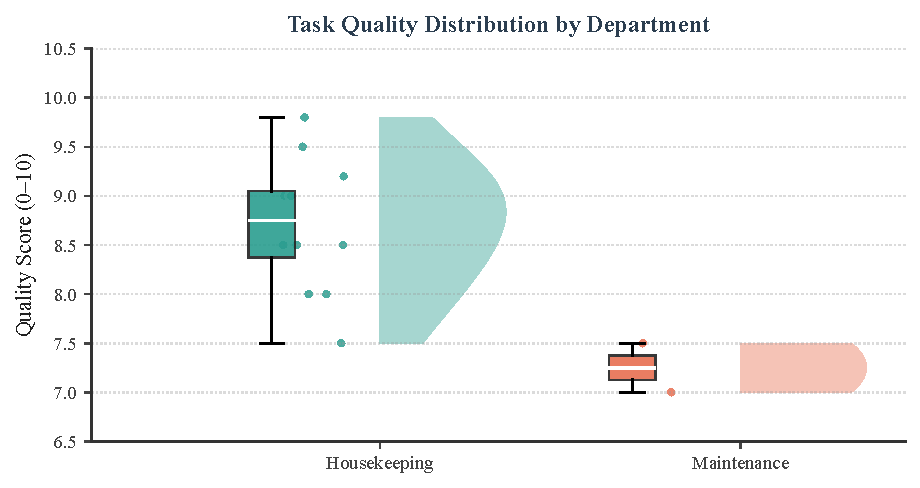
\includegraphics[width=0.70\linewidth]{fig5_raincloud_quality.pdf}
\caption{Raincloud plot of \texttt{Task\_Log.Quality\_Score} by department. The Housekeeping cloud is denser and skews to 9+; Maintenance shows a wider, lower distribution -- a candidate signal for staff training and a hiring case for a second technician.}
\label{fig:raincloud}
\end{figure}

\begin{figure}[H]
\centering
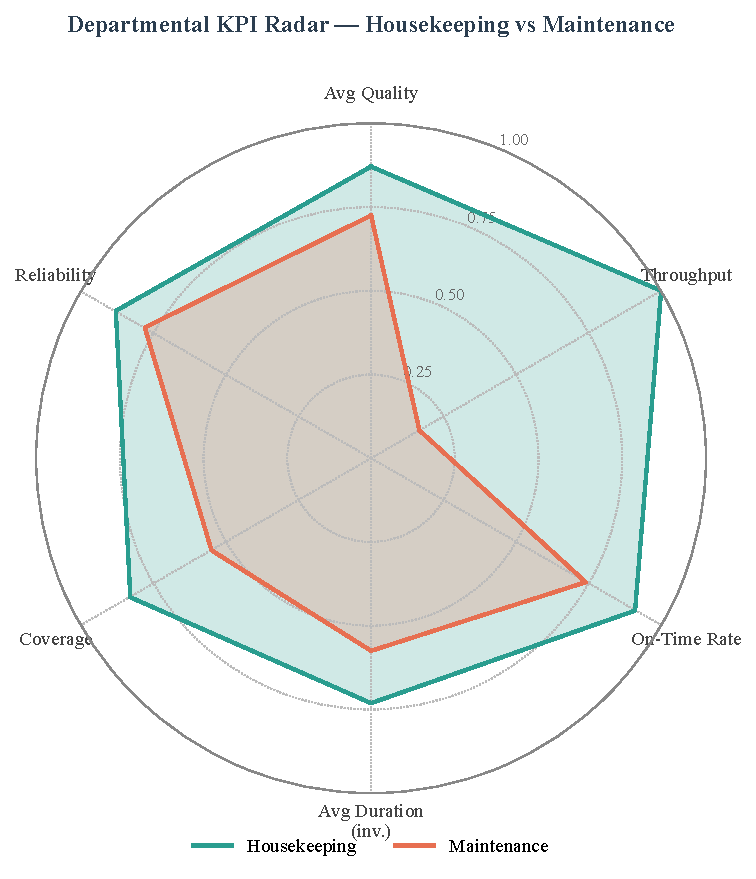
\includegraphics[width=0.55\linewidth]{fig10_radar_dept_kpi.pdf}
\caption{Departmental KPI radar (normalised). Housekeeping leads on Quality and Throughput while Maintenance carries the longest mean Duration -- the same signal Q6/Q8 emit numerically.}
\label{fig:radar}
\end{figure}

\textbf{Finding F5} is made plain by Figure~\ref{fig:payments}: 87.6\% of
payment volume is Completed, 8.1\% Refunded and 4.2\% Pending, while
Credit-Card transactions dominate the premium right tail (ARPU \$1{,}264 vs
Cash \$136). The CDF in Figure~\ref{fig:cdf} closes the loop: roughly 60\%
of bookings fall under \$500, but the top 20\% of bookings absorb the bulk
of payment volume -- exactly the cohort most exposed when card rails fail.

\begin{figure}[H]
\centering
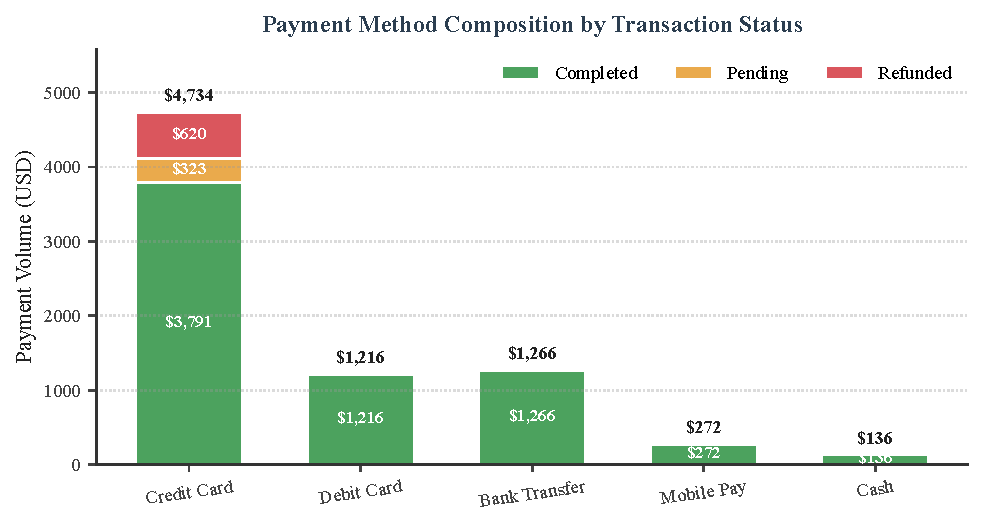
\includegraphics[width=0.78\linewidth]{fig9_stacked_bar_payments.pdf}
\caption{Stacked breakdown of payment volume by status and method (Q7/Q9). 12.37\% of finalised revenue sits in Pending or Refunded states; Credit-Card dominates the premium right tail.}
\label{fig:payments}
\end{figure}

\begin{figure}[H]
\centering
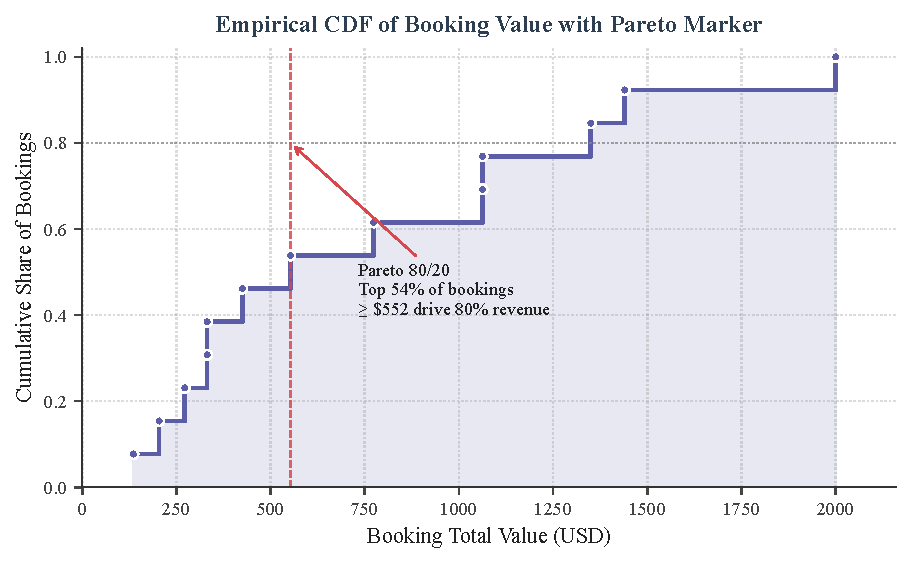
\includegraphics[width=0.65\linewidth]{fig11_cdf_booking_value.pdf}
\caption{Empirical CDF of completed booking value. The flat tail above \$1{,}500 is where revenue concentration meets cancellation risk -- the structural reason Finding F2's \$2{,}480 loss matters.}
\label{fig:cdf}
\end{figure}

The remaining queries close the loop: Q2 occupancy (Deluxe Suite first); Q3
pricing impact (5 rows matched Christmas $+80\%$, mirroring \textbf{F3}'s
$+2.20\%$ net premium); Q9 dashboard view (18 rows); Q10 cancellation watch
(Jan 2026 flagged \textsc{Critical} at 50\%); Q12 overlap audit (0 conflicts).

% ============================ 6. Innovation ============================
\section{Innovation: Database-Driven Pricing Agent}

We pair the schema with a Python \emph{Pricing Agent} that consults the
database in real time. For a target date and room type the agent reads the
highest-priority active rule from \textsc{Dynamic\_Pricing\_Rule}, computes
the occupancy rate from \textsc{Booking\_Room\_Detail}, and returns
\begin{equation*}
P_\text{final} \;=\; P_\text{base} \;\times\; m_\text{rule} \;\times\; f_\text{occ},
\qquad f_\text{occ} \in \{0.85,\,1.0,\,1.10,\,1.30\}.
\end{equation*}

Figure~\ref{fig:lollipop} summarises the four rules currently loaded.
\textbf{Finding F3} bears directly on this design: aggregating actual versus
base rate across non-cancelled details shows only a +2.20\% net premium,
because the weekday discount (-\$1{,}230 across 12 details) almost cancels
the Christmas surcharge (+\$1{,}496 across 3 details). The remedy is a
structural one -- shorten the 5-month weekday window or tighten its
eligibility -- and because the rule lives in a row, not in code, that remedy
is a single \texttt{UPDATE}.

\begin{figure}[H]
\centering
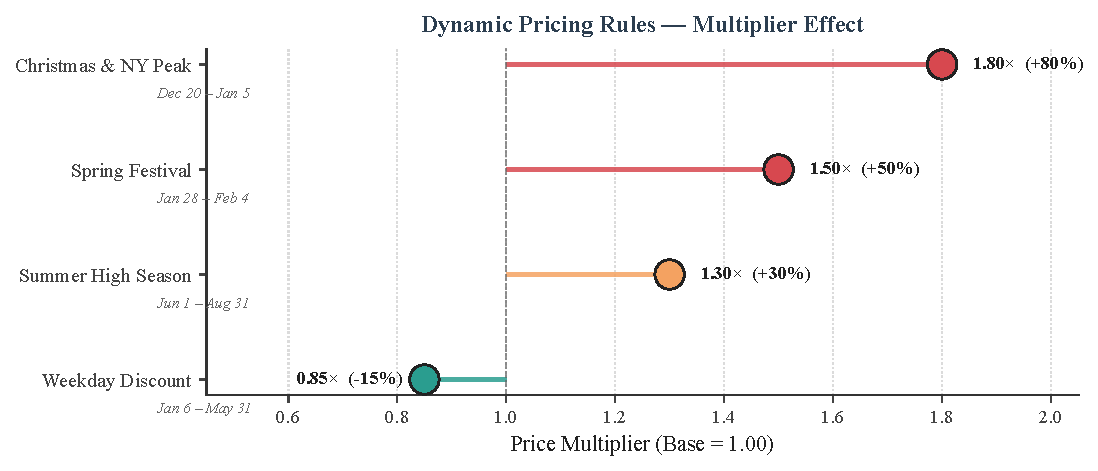
\includegraphics[width=0.72\linewidth]{fig6_lollipop_pricing.pdf}
\caption{The four dynamic-pricing rules currently loaded. Christmas/NY drives the strongest surge ($+80\%$); the weekday discount ($-15\%$) is wide enough to nearly neutralise the seasonal upside.}
\label{fig:lollipop}
\end{figure}

Figure~\ref{fig:agentflow} traces the agent's decision flow through the
database. The agent's intelligence lives in the data layer: changing a row in
\textsc{Dynamic\_Pricing\_Rule} immediately re-targets pricing without code
redeployment -- exactly the separation a BCNF schema is built to enable.

\begin{figure}[H]
\centering
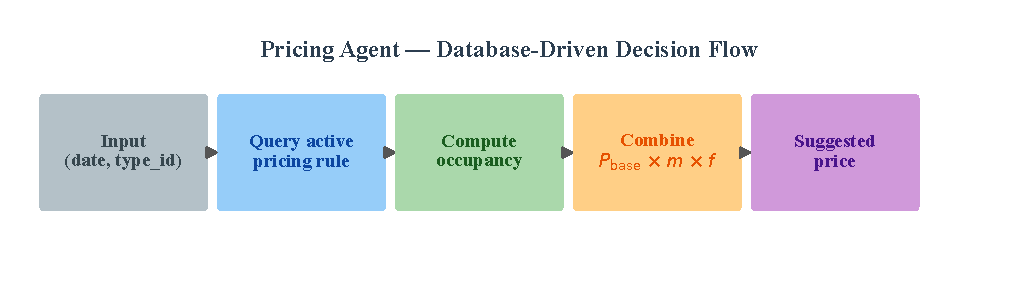
\includegraphics[width=0.85\linewidth]{fig7_agent_flow.pdf}
\caption{Pricing-Agent decision flow. The agent reads rules and occupancy from the database, computes the final price and returns the recommendation -- a closed loop entirely mediated by SQL.}
\label{fig:agentflow}
\end{figure}

% ============================ 7. Conclusion ============================
\section{Conclusion}
The system satisfies every basic requirement of Scenario~2 and adds five
operationally grounded extensions. The schema is normalised to BCNF, exercised
by 12 queries that reference all 11 relations, and the sample data is dense
enough to surface five managerial findings (ARPU vs.\ points decoupling, peak
cancellation concentration, weekday-discount erosion, departmental quality
gap, and at-risk payment volume) without inflating row counts beyond a
defensible test instance. The Pricing Agent then demonstrates the payoff of a
well-normalised design: the database is not passive storage but the substrate
of an autonomous, single-\texttt{UPDATE}-tunable decision loop.

\end{document}
